\documentclass[12pt,a4paper]{article}
\usepackage[utf8]{inputenc}
\usepackage[T1]{fontenc}
\usepackage{setspace}
\usepackage{amsmath}
\usepackage{amsfonts}
\usepackage{amssymb}
\usepackage{graphicx}
\usepackage{times}
\usepackage{tabularx,ragged2e,caption} 
\usepackage[table]{xcolor}
\usepackage[sort&compress, numbers]{natbib}
\usepackage{hyperref,url}
\usepackage{caption}
\usepackage{array}
\usepackage{subcaption}
\usepackage{makecell}
\usepackage[nottoc]{tocbibind}
\usepackage{multirow}
\usepackage{multicol}
\usepackage{float}
\newcommand{\angstrom}{\text{\normalfont\AA}}

\usepackage[left=2.50cm, right=2.00cm, top=2.00cm, bottom=3.00cm]{geometry}

\begin{document}
\begin{titlepage}
\begin{center}
    \fontsize{24}{24}\selectfont \textbf{ SUPERCONDUCTIVITY OF THE TaSb\textsubscript{2} BY APPLYING HIGH PRESSURE}
\end{center}

\vspace{1cm}

\begin{center}
    {\large\textbf{A Research Proposal \vspace{0.2cm}\\ Submitted to Central Department of Physics, T.U., Kirtipur, Nepal\\ in Partial Fulfillment of the Requirement for the \\ Master's Degree of Science in Physics}}
\end{center}

\begin{figure}[ht]
    \centering
    
\includegraphics[scale=0.65]{tu .png}
\end{figure}

\vspace{1cm}
\begin{center}
    \textbf{{\large Submitted By}\\
    .............................................\vspace{0.3cm}\\
    {\LARGE Ricky Rai }\\}
    \large \textbf{Roll No.: 88}\\
    \large \textbf{\today}
\end{center}
\end{titlepage}

\pagenumbering{gobble}
\pagenumbering{roman}
\begin{spacing}{1}
    \tableofcontents
\end{spacing}
\pagebreak


\newpage
\pagenumbering{arabic}
\vspace*{\fill}

\section{Introduction}
\noindent
\subsection{superconductivity}

During 1911, while cooling mercury inside the cryostat(it was filled with liquid helium), Heike Kamerlingh Onnes found that  mercury exhibits zero resistance \cite{onnes1911}at critical temperature T$_c$=4.2K. This is the first time in human history that a superconductor was found. At that time he was awarded the Nobel Prize. Later on in 1933, it was observed that along with zero-resistivity, superconductor behavior shows that magnetic flux lines are also expelled from it, which was first observed by Meissner and Ochen \cite{meissner1933}. It tells us that superconductors exhibit perfect diamagnetism. It is called Meisner effect.
\begin{figure}[ht]
    \centering
    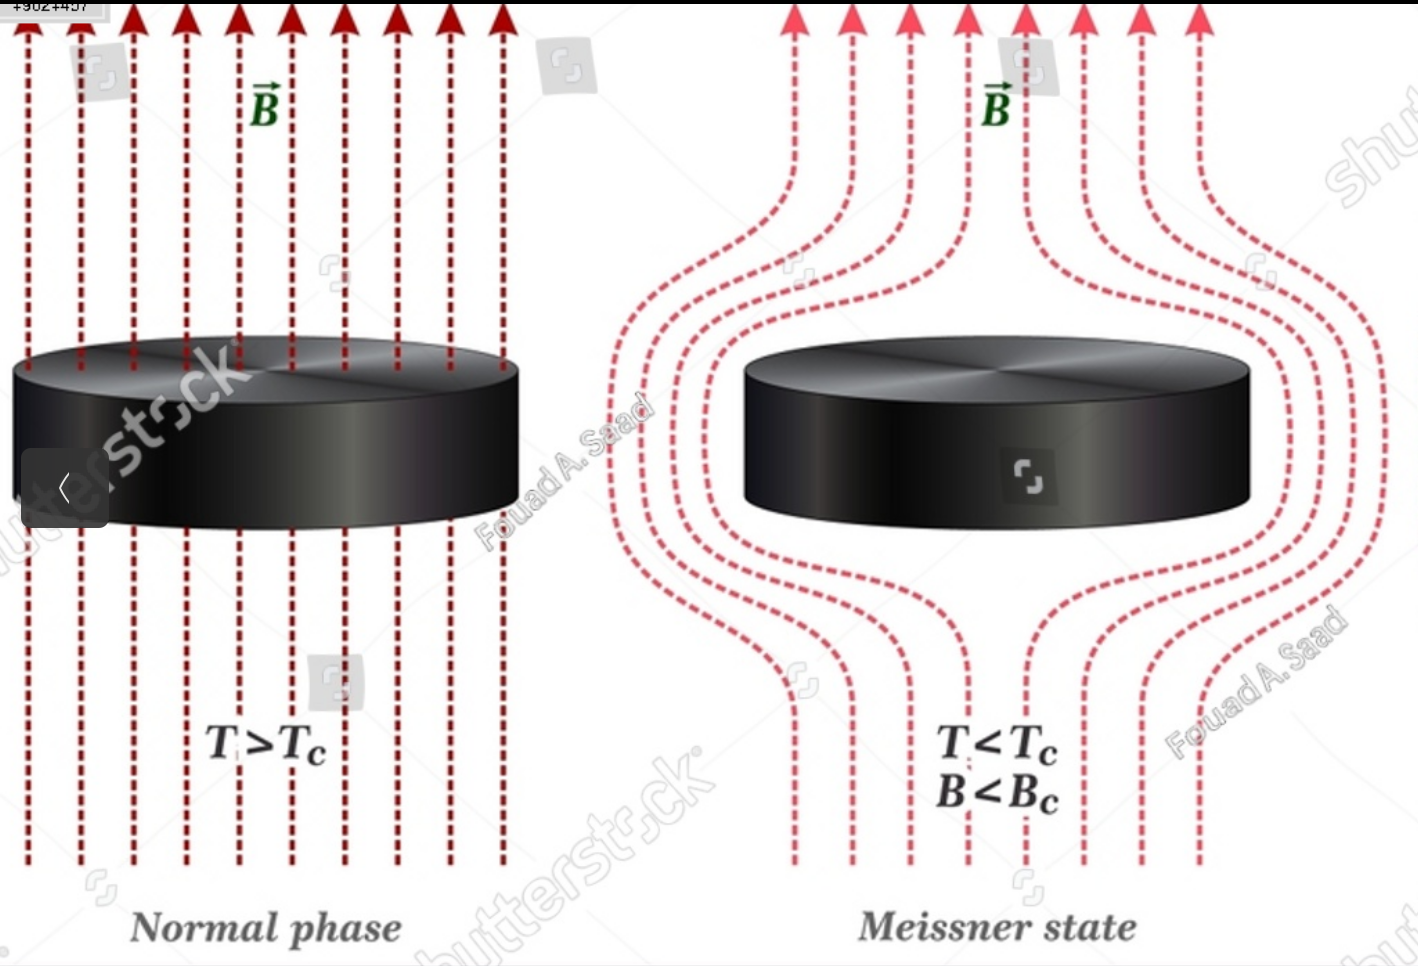
\includegraphics[scale=0.20]{Messner.png}
    \caption{The meissner effect\cite{shutterstockSuperconductors}}
\end{figure} 
But it was all experimental observation, and it still lacks the theoretical physics behind it. This mystery was carried until 1957, when three professors, Barden, Cooper, and Schrieffer, combinedly proposed a theory known as BCS, renamed after the three professors, that incorporated a strong reason behind the existence of superconductors and unraveled the mystery of it and gave the concept of Cooper pairs\begin{figure}[h!]
    \centering
    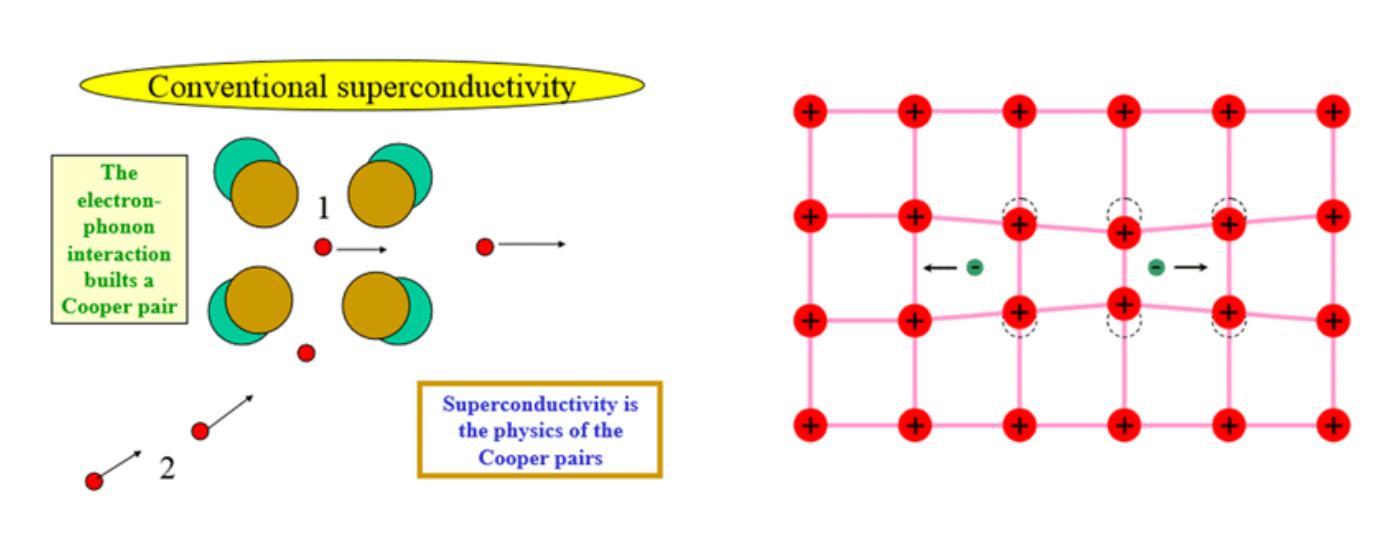
\includegraphics[scale=0.30]{PAiR.png}
    \caption{Cooper pairs\cite{rampino2015cooper}}
\end{figure}  \cite{bcs1957}.



The central objective of this thesis is to explore the pressure-induced superconducting behavior of TaSb\textsubscript{2} using first-principles density functional theory (DFT) calculations. We aim to investigate the electronic band structure, phonon dispersion, density of states (DOS), and electron-phonon coupling under varying pressure conditions. Specifically, we intend to analyze how pressure modifies the Fermi surface, alters the density of states at the Fermi level, and influences the superconducting transition temperature \(T_c\) using the Allen-Dynes modified McMillan formula:
\[
T_c = \frac{\omega_{\log}}{1.2} \exp \left[ \frac{-1.04(1 + \lambda)}{\lambda - \mu^*(1 + 0.62\lambda)} \right]
\]
where \(\lambda\) is the electron-phonon coupling constant, \(\omega_{\log}\) is the logarithmic average phonon frequency, and \(\mu^*\) is the Coulomb pseudopotential.
\subsection{Crystal structure of TaSb2}



Tantalum diantimonide (TaSb\textsubscript{2}) forms a single-crystal system with the space group \textit{C2/m} (No.~12). The unit cell's dimensions are approximately $a = \SI{10.35} {\angstrom}$, $b = \SI{3.70} {\angstrom}$, $c = \SI{8.38} {\angstrom}$, and $\beta = 120.5^\circ$. Each Ta atom in this structure is coordinated by eight Sb atoms, creating a deformed polyhedral environment. Strong covalent interactions are indicated by the Ta--Sb bond lengths, which range from \SI{2.87} {\angstrom} to \SI{3.01} {\angstrom}. The compound exhibits a layered and anisotropic three-dimensional structure, which influences its semimetallic or topological characteristics under various external conditions such as applied pressure or doping~\cite{jung2024pressure}.

\begin{figure}[h!]
    \centering
    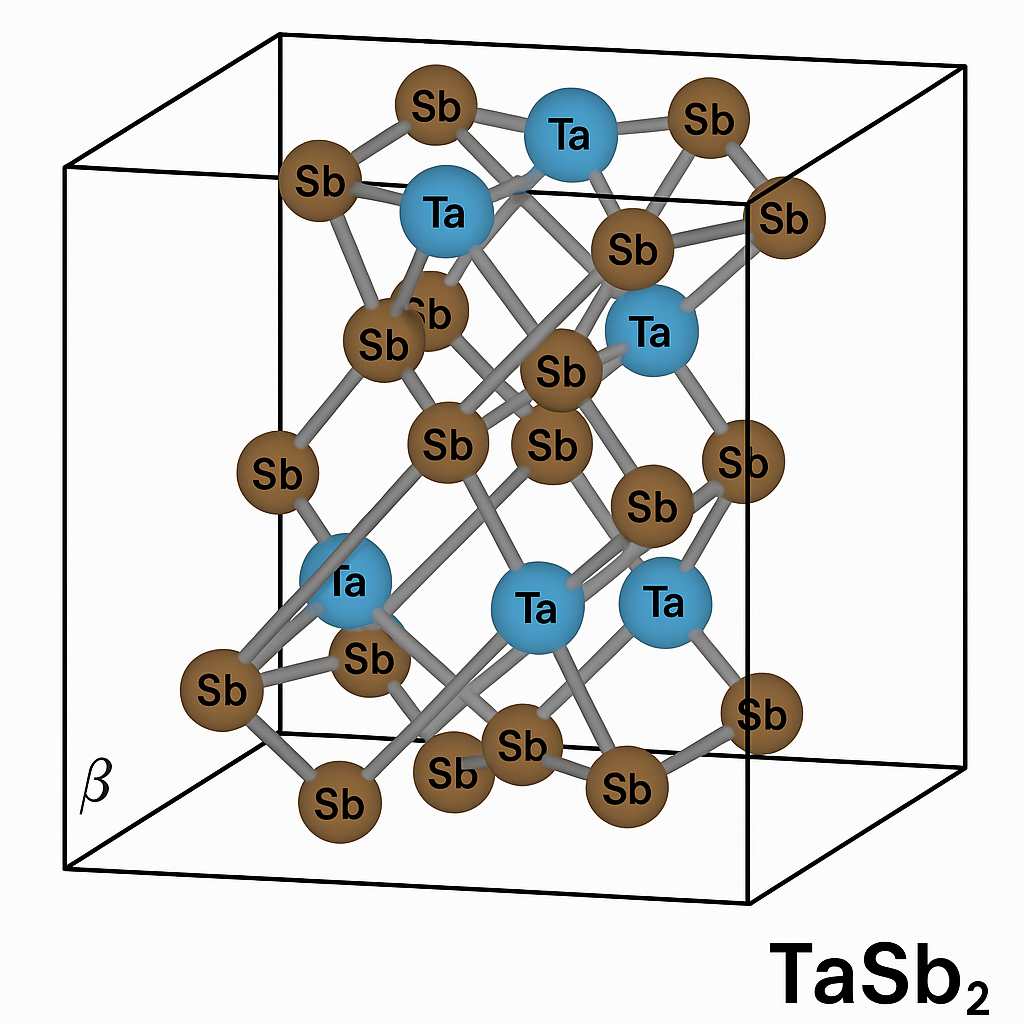
\includegraphics[scale=0.30]{cryst.png}
    \caption{Crystal structure of TaSb2\cite{openai2025tasb2}}
\end{figure}  






\section{Literature Review}

\subsection{Introduction to High-Temperature Superconductors}

High TC superconductor has always been fascinating idea, especially for commercial purpose. The commercial purpose plays the vital role to lead human races for the study of superconductor. But it's the BCS theory which sets the limit that no any material could achieve superconductivity property beyond the absolute temperature 30 Kelvin. However in 1986, the first high-temperature superconductor was discovered by Bednorz and Müller, namely LaBaCuO (LBCO) from the type of copper oxide family which which not only disobey the BCS theory, but also closes the chapter of conventional superconductor.
\subsection{Study on high pressure Superconductivity}

The concept of a high-pressure superconductor was first proposed in the latter half of the 20th century. Researchers started looking at these fascinating fields. According to a 2015 article, hydrogen sulfide (H$_3$S) demonstrated superconductivity properties at temperatures close to room temperature. 203 Kelvin, or about 150 GPa of pressure, shattering all prior records\cite{drozdov2015}. This is the area of high-pressure superconductivity that interests me. The research on pressure-induced superconductivity in NbAs$_2$ sparked my curiosity in investigating a novel compound from the same family, TaSb$_2$, which may exhibit comparable behavior under high pressure and is discussed in this study\cite{nbas2-pressure-sc}.Since our material will exhibits superconductivity only due to pressure.Here the insight how pressure vs lattice constant and volume per atom graph works.
\begin{figure}[h!]
    \centering
    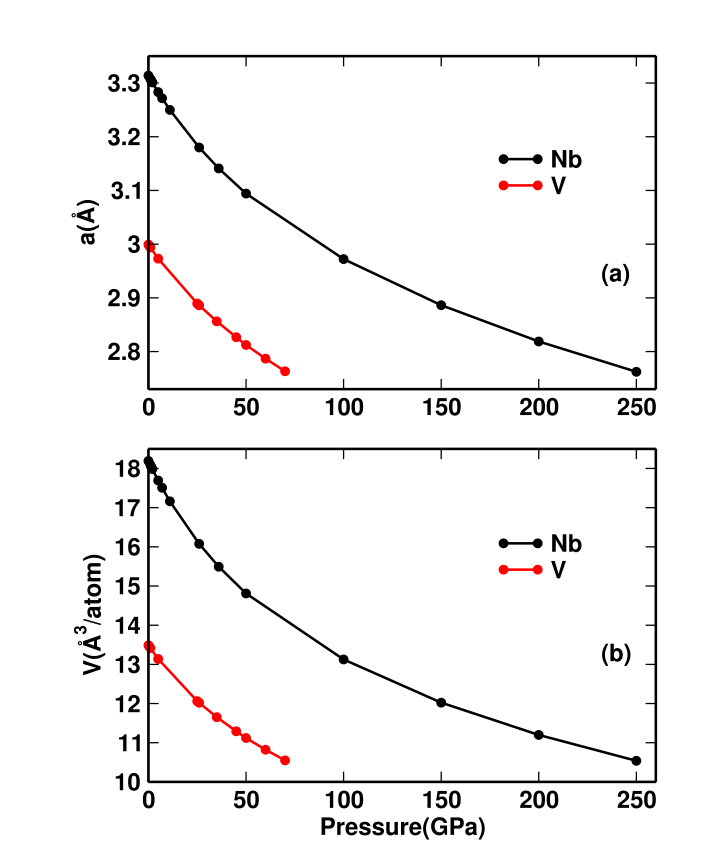
\includegraphics[scale=0.35]{himal oli.png}
    \caption{pressure vs (a)lattice constant and (b)Volumer per atom of V and Nb\cite{oli2024first}}
\end{figure}  



\newpage
\subsection{Comparison with related compound}
Both TaSb\textsubscript{2} and NbAs\textsubscript{2} belong to a class of substances known as transition metal dipnictides. They are recognized for their intriguing electrical characteristics and have comparable structural structures. However, they behave very differently in the context of superconductivity.

Superconductivity in the case of TaSb\textsubscript{2}, either under normal conditions or under high pressure, has not been clearly reported\cite{ta-review}. The majority of existing research focuses on its topological aspects and transport characteristics. While various research have investigated the behavior of TaSb\textsubscript{2} under pressure, none have demonstrated that it transforms into a superconductor. This raises the question of whether TaSb\textsubscript{2} can exhibit superconductivity in previously untested circumstances, such as increased pressure or various tuning methods.

However, under pressure, NbAs\textsubscript{2} has already demonstrated superconductivity\cite{nbas2-pressure-sc}. With a transition temperature (Tc) of roughly 2.6 K, researchers discovered that NbAs\textsubscript{2} begins to behave like a superconductor when pressure is raised to about 12.8 GPa. It's interesting to note that this occurs without causing any alteration to its crystal structure, so even as it turns superconducting, the fundamental atomic arrangement remains unchanged. NbAs\textsubscript{2} is therefore a promising material for future research, particularly since it may possibly be related to topological superconductivity.

In conclusion, TaSb\textsubscript{2} has not yet demonstrated the ability to behave as a superconductor under pressure, but NbAs\textsubscript{2} has already been demonstrated to do so. This makes TaSb\textsubscript{2} a promising candidate for additional study to see if it can likewise be made into a superconductor through the use of high pressure or other techniques.
\newpage
\section{Objectives}
\subsection{General Objective}
\begin{itemize}
     To explore the emergence of superconductivity in TaSb$_2$ under pressure through comprehensive first-principles simulations.
\end{itemize}

\subsection{Specific Objectives}
\begin{itemize}
    \item To investigate the evolution of the electronic band structure and density of states of TaSb$_2$ across a range of applied pressures.
    \item To determine the phonon dispersion spectra and examine the dynamical stability of the compound under varying pressure conditions.
    \item To quantify the strength of electron-phonon interactions and estimate the critical temperature for superconductivity using ab-initio calculations.
    \item To understand the pressure-dependent behavior of superconducting characteristics and identify the threshold pressure necessary for superconductivity onset in TaSb$_2$.
\end{itemize}


\pagebreak




\section{Theory and Methodology}
\subsection{Theory}

\subsubsection{BCS Theory}


The BCS theory was the first successful microscopic explanation of superconductivity. According to this theory, when the temperature is above a certain critical value, the thermal energy is too high for electrons to form stable Cooper pairs. But as the temperature goes down, vibrations in the lattice (called phonons) can create an attraction between electrons. This attraction helps electrons to pair up by overcoming their natural repulsion. These pairs are called Cooper pairs\cite{bcs1957}.

The energy needed to break a Cooper pair is called the energy gap, and it is given by the following formula:

\[
\Delta = \frac{2\hbar \omega}{\exp\left(\frac{1}{N(0)V_0}\right) - 1}
\]

Here, \( \omega \) is the angular frequency of phonons exchanged between two electrons, \( N(0) \) is the density of single-electron states at the Fermi level (for one spin direction), and \( V_0 \) is the attractive interaction between electrons.

For the weak coupling case, where \( N(0)V_0 \ll 1 \), the equation becomes:

\[
\Delta = 2\hbar \omega \exp\left(-\frac{1}{N(0)V_0}\right)
\]

This final equation gives the energy needed to break the Cooper pair in the weak coupling limit.
\subsubsection{ELecrtron-phonon coupling(EPC)}


The electron-phonon coupling constant \( \lambda \) is defined as:

\[
\lambda = 2 \int_0^{\infty} \frac{\alpha^2F(\omega)}{\omega} \, d\omega
\]

where \( \alpha^2F(\omega) \) is the Eliashberg spectral function, and \( \omega \) is the phonon frequency \cite{grimvall1981}.

\subsubsection{Allen-Dynes equation}



The superconducting transition temperature \( T_c \) can be estimated using the Allen-Dynes-modified McMillan formula:

\[
T_c = \frac{\omega_{\log}}{1.2} \exp\left(
\frac{-1.04(1+\lambda)}{\lambda - \mu^*(1 + 0.62\lambda)}
\right)
\]

\noindent where:
\begin{itemize}
    \item \( T_c \): Superconducting critical temperature (K),
    \item \( \omega_{\log} \): Logarithmic average of phonon frequencies,
    \item \( \lambda \): Electron-phonon coupling constant,
    \item \( \mu^* \): Coulomb pseudopotential (typically \( \mu^* \approx 0.10 \)).\\
    \par
    \vspace{2mm}
    Here the value of effective coulomb repulsion is typically based on empirical formula observations and theoretical considerations.Large   \( \mu^* \) would indicate strong electron-electron repulsion dominating cooper pair.So for conventional superconductors it's value i.e.  \( \mu^* \)=0.1 is found to strike balance giving reasonable T$_c$
    
\end{itemize}

This equation is widely used in first-principles calculations of superconductors to relate microscopic quantities to the critical temperature. It is particularly effective for phonon-mediated superconductors.

As derived and discussed in \cite{allen1975}, this formula improves upon the original McMillan expression by accounting more accurately for strong coupling effects.
\pagebreak



\section{Methodology}
\subsection{Density Functional Theory (DFT)}



One popular technique in materials science for forecasting the behavior of atoms, molecules, and solids is density functional theory, or DFT. By concentrating on the electron density—the distribution of electrons within the material—it aids researchers in their investigation of the electrical characteristics of these systems.

DFT suggests that ground state attributes can be determined without knowing the entire many-body wavefunction. Alternatively, the electron density \( \rho(\mathbf{r}) \), a three-dimensional scalar function, can be used to compute the total energy of a system \cite{hohenberg1964inhomogeneous}. DFT tackles the intricate many-body problem by using quantum mechanical concepts. 

Kinetic energy and electron-electron interactions are approximated as the precise link between ground state energy and electron density is not known. Self-consistent equations like the Hartree and Hartree-Fock approaches were produced by Hohenberg and Kohn's introduction of an approximation technique appropriate for high-density systems \cite{hartree1928wave,fock1930naherungsmethode}. The ground state energy can be found by solving these equations using variational methods.

This study uses \textit{Quantum ESPRESSO}, a freely available program based on DFT, plane waves, and pseudopotentials, to perform electronic structure and related computations. \textit{Quantum ESPRESSO} is used to do first-principles DFT simulations in order to investigate the band structure, phonon density of states, and electron-phonon coupling constant (\( \lambda \)) of sodium-intercalated molybdenum carbide \cite{giannozzi2009quantum}.


\subsection{Methodology for TaSb\textsubscript{2} Under Pressure}

% Structural optimization and calculations:
We perform all simulations using Quantum ESPRESSO \cite{giannozzi2009quantum}, and phonon properties using Density Functional Perturbation Theory (DFPT) \cite{baroni2001phonons}.

% Tc calculation
Critical temperature is estimated using the Allen-Dynes modified McMillan formula \cite{allen1975transition}.

\subsection{Software and Tools}
The following tools are commonly used for implementing machine learning techniques:

\begin{itemize}
    
    \item Quantum Expresso
    \item Vesta, XCRYSDen
    \item GNU plot,Xm GRace
    
\end{itemize}


\newpage
\section{Expected Outcomes}





Through the determination of the superconducting transition temperature (\(T_c\)) at different pressures, this study seeks to investigate the pressure-induced superconductivity in TaSb$_2$. We'll look into how pressure affects superconductivity and determine the pressure levels where it manifests or becomes stronger.

Additionally, the study will investigate the alterations in electronic structure, density of states (DOS), and phonon dispersion under pressure in an effort to identify the mechanisms underlying TaSb$_2$ superconductivity. We will also compute the electron-phonon coupling constant (\( \lambda \)) and how it relates to \(T_c\).

The theoretical predictions will be verified by comparing our findings with the existing experimental data. In the absence of such data, our results will offer a theoretical insight into TaSb$_2$. An important component of our master's thesis on superconductivity in TaSb$_2$ will be this work.

\section*{Acknowledgement}

I want to sincerely thank Professor \textbf{Dr. Narayan Prasad Adhikari} , my supervisor, for his important advice and support throughout the writing of my thesis proposal.
His wise recommendations have greatly influenced the course of the investigation into superconductivity in the compound TaSb$_2$. I sincerely appreciate his guidance and assistance.


\vspace{0.5cm}


\vfill
\pagebreak



\section{Timeline}
To complete the work in a given time, work plan is needed. Work plan helps to utilize the time effectively to finish the work in time. The work plan for this purposed work is shown in table.\\\\\\\
\setlength{\tabcolsep}{17pt}
\begin{tabular}{|c|c|c|c|c|c|c|}
	
	\hline
	\multirow{2}{*}{\textbf{Work}} &\multicolumn{6}{|c|}{\textbf{Time Duration (in months)}}	\\	
	\cline{2-7}
	{}	&\textbf{1-2 }&	\textbf{3-4}&\textbf{	5-6 }&	\textbf{7-8 }&\textbf{9-10}&\textbf{10-11}\\
	
	\hline
	\makecell{	\textbf{Review of}\\\textbf{Literature}}&	\cellcolor{red!100}& \cellcolor{red!100}& & &&\\
	\hline
	\makecell{\textbf{Software} \\\textbf{Familiarization}}& &	\cellcolor{blue!100}&\cellcolor{blue!100}&&&\\
	\hline
	\makecell{\textbf{Data enumeration \&} \\ \textbf{calculation}}&&&	\cellcolor{green!100}&\cellcolor{green!100}&&\\
	\hline
	\makecell{\textbf{Data Analysis} \textbf{\&} \\\textbf{Interpretation}}&&&\cellcolor{black!100}&	\cellcolor{black!100}&\cellcolor{black!100}&\\
	\hline
	\makecell{\textbf{Thesis writing} \textbf{\&} \\ \textbf{Documentation}}&&&&&	\cellcolor{cyan!100}&\cellcolor{cyan!100}\\
	\hline
	
\end{tabular}\\\\\\\\\

	\pagebreak
	\bibliographystyle{unsrt}
	\bibliography{References}
     \pagebreak 

	\section*{Supervisors}
	\textbf{\underline{Supervisor:}}\vspace*{0.4cm}\\
 
	\ldots\ldots\ldots\ldots\ldots\ldots\ldots\ldots\ldots\ldots\ldots\ldots\ldots\\ \noindent \textbf{{Prof. Dr. Narayan Prasad Adhikari}}\\ \textit{Central Department of Physics}\\\textit{Tribhuvan University} \\{\textit{Kathmandu,Nepal}}\\
	
	\noindent 

 
	\noindent \textbf{\underline{Co-Supervisor:}}\vspace*{0.4cm}\\
	\ldots\ldots\ldots\ldots\ldots\ldots\ldots\ldots\ldots\ldots\ldots\ldots\ldots\\ \noindent \textbf{{.............}}\\ \textit{ .............Campus}\\\textit{Tribhuvan University} \\{\textit{Kathmandu,Nepal}}
	
	\pagebreak

\end{document}
